\section{Scientific Methodology}
\label{sec:scientific_method}
%\red{Youyi}\\

Seismic tomography involves the construction of images of Earth's interior by
minimizing a predefined misfit function involving observed and synthetic data. Typically, 
seismic signals are generated by a wide variety of sources and recorded by a
set of receivers as time series of a physical quantity. Sources can be either 
passive (e.g., earthquakes, ambient noises) or active (e.g., nuclear explosions, 
air guns, etc.). In the most common cases, the receivers record a quantity, such as displacement, 
on vertical and/or horizontal components. In the past decades, 
seismic datasets have grown very fast with accumulating sources and a
dramatic increase in the number of receivers (e.g., cross-continental array
deployments in passive seismology, 3D surveys in active source seismology). Such
growth provides more information to constrain the model in greater details, but
also poses a challenge for processing massive seismic data. In addition to
the data deluge, a numerical solver capable of accurately simulating seismic wave
propagation is very important for tomography to achieve higher resolution. 
To solve the (an)elastic or acoustic wave equation in realistic 3D models, a spectral-element
method~\cite{KoTr99, KoTr02a, KoTr02b} is used to achieve
high accuracy for realistic Earth models in complex geometries.
Since the most computationally expensive part of a tomographic inversion
involves wavefield simulations, excellent performance of the solver is crucial,
as discussed in Section~\ref{sec:solver}.

\begin{figure}[h]
\begin{center}
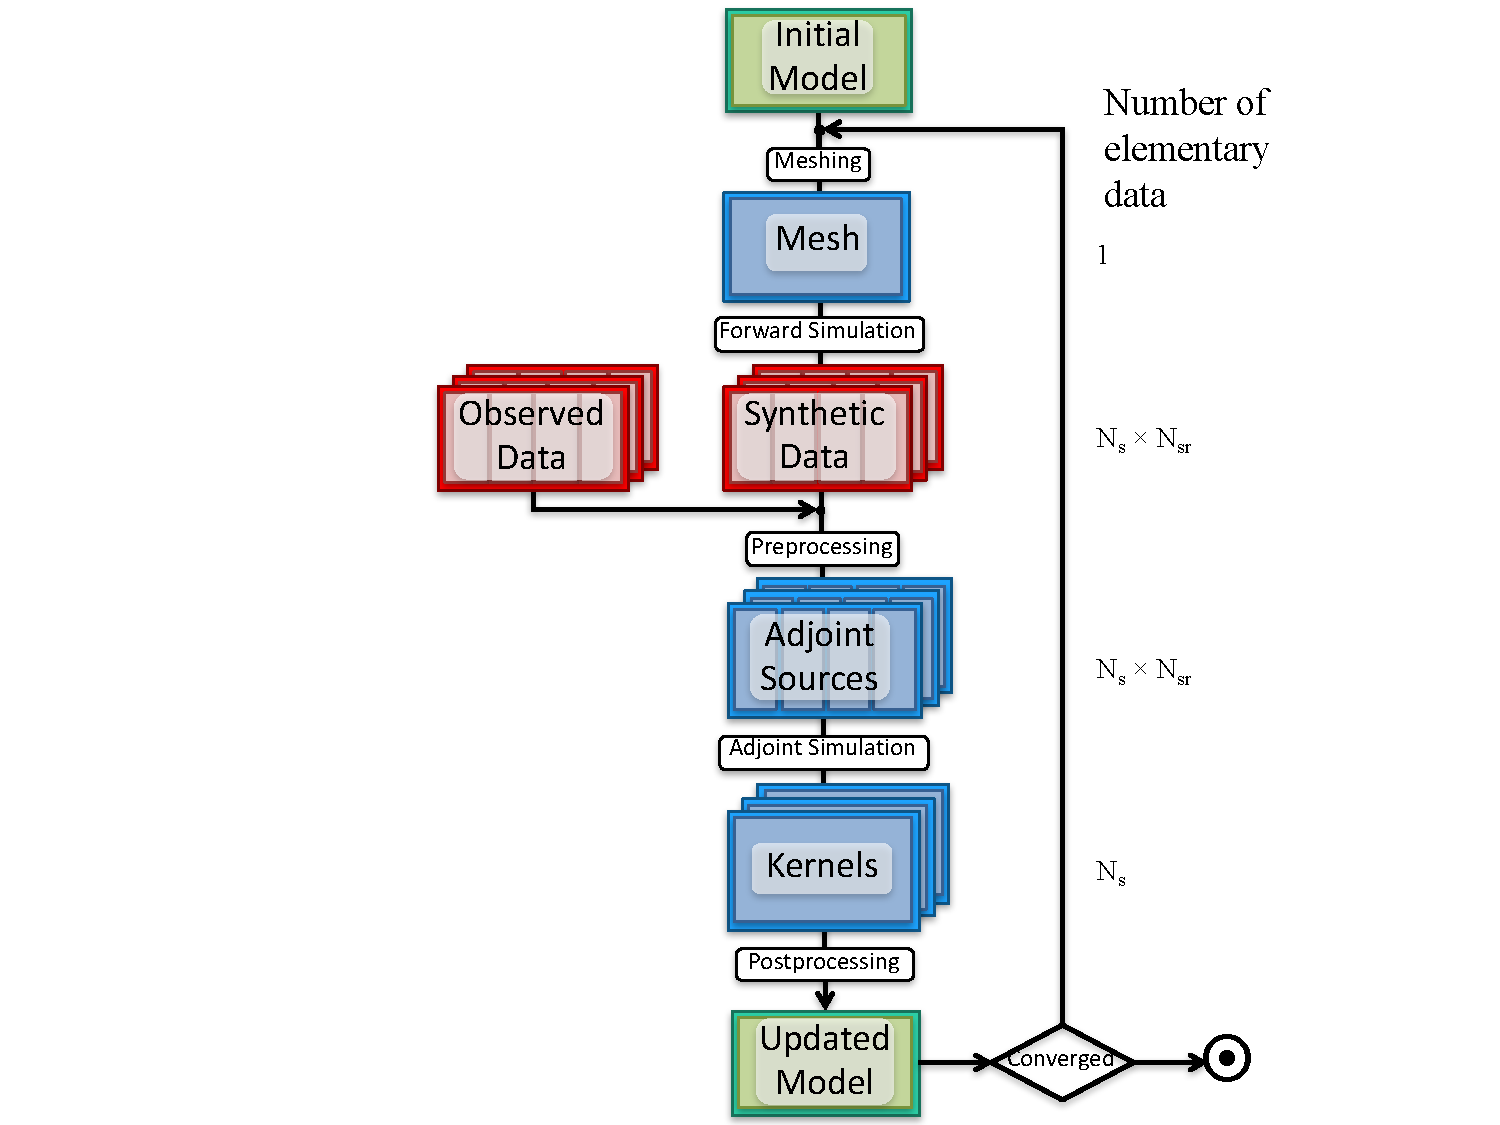
\includegraphics[width=\columnwidth]{ch-workflow/figures/seismic_data_workflow.pdf}
\caption{General adjoint tomography workflow. The focus is on the data
involved in each step. Seismic data are depicted by red boxes and for each of
the $N_{s}$ seismic events they are recorded by $N_{sr}$ receivers.
Computational data are represented by green and blue boxes. The amount of
elementary data varies depending on the workflow stage and can eventually be
grouped into a smaller number of files.}
\label{fig:seismic_data_workflow}
\label{default}
\end{center}
\end{figure}
%

%Using data from 253 earthquakes and adjoint tomography technique, we generated 
%a global Earth model, GLAD-M15 ~\cite{Bozdag2016}.  To further improve the resolution 
Using data from 253 earthquakes and adjoint tomography technique, we generated model
GLAD-M15~\cite{bozdaug2016global}, the first Earth model where forward and Fr\'echet
derivative calculations were performed numerically in 3D background models.  To
further improve the resolution of this model, we have expanded the dataset to
1,000 earthquake, and will eventually include all available earthquakes (Mw
5.0-7.0) on the global scale (more than 6,000 as of 2016). Inverting 
such a large dataset requires optimizing I/O
performance within data processing and simulations as well as efficient management
of the entire workflow. Preparing for exascale computing in seismic
tomography, we address the bottlenecks we encounter in our current adjoint
tomography studies and discuss possible solutions. A
typical adjoint tomography workflow is shown in
Figure~\ref{fig:seismic_data_workflow}.
It involves three major
stages: (1) calculating synthetic seismograms and pre-processing observed and synthetic data, 
(2) calculating the gradient of the misfit function
(the Fr\'echet derivatives), and (3) post-processing and updating the model.

The pre-processing stage is dedicated to assimilating data: (1) signal
processing (i.e., tapering, re-sampling, filtering, deconvolving the instrument
response, etc.), (2) window selection to determine the usable parts of
seismograms according to certain criteria by comparing observed and simulated
seismograms; and (3) making measurements in each window and computing
the associated adjoint sources~\cite{Tromp2005, tape2009adjoint, Zhu2009, Luo2013}. 
The pre-processing stage can easily involve dealing with millions of seismograms 
and has become a bottleneck in tomographic inversions.
Although some groups have their own data formats, the Seismic Analysis Code (SAC) format 
has been the main seismic data format for earthquake seismology. Seismic data
in SAC files are single time series stored independently for each component of each receiver, along with 
limited metadata as header. For large scales studies, this format produces
severe I/O traffic in data processing and numerical simulation due to the large
numbers of files to be dealt with.  
An Adaptable Seismic Data Format (ASDF) has been developed as an alternative 
to SAC\@. It enables flexible data types and allows storing large data in a single file 
through its hierarchical organization. We illustrate the advantages of this new data
format in Section~\ref{sec:asdf}.

Computing the gradient of the misfit or objective function is accomplished through
the interaction of a forward seismic
wavefield with its adjoint wavefield; the latter is generated by back-projecting
seismic measurements simultaneously from all receivers~\cite{Tarantola1984}.
This procedure requires two numerical
simulations for each source: one for the forward wavefield from the source to
the receivers, and another for the adjoint wavefield from all the receivers to the
source. The simulations are run for each source, resulting in \emph{event kernels},
and the gradient of the misfit function is simply the sum of all event kernels.
Between forward and adjoint simulations, we need to store a vast amount of
wavefield data to account for the full attenuation of seismic waves in an anelastic
Earth model.  
For thousands of events, the I/O approach we used to efficiently
calculate the kernels is discussed in Section~\ref{sec:computational_data}.
In the post-processing stage, the gradient is pre-conditioned and
smoothed.  Based upon the gradient, a model update is obtained using a
conjugate gradient or L-BFGS~\cite{Nocedal1980} optimization scheme. Usually,
tens of iterations have to be performed to obtain a stable model, and in each iteration
we have to process data, and run forward and adjoint simulations for thousands of
events. At each stage, an additional complication is the necessity to check
results and relaunch jobs when failure occurs. Manually handling the procedures
described above is difficult because of the size of the dataset and also because of
the distributed resource environment.
Therefore an efficient scientific workflow
management system is needed, and various options will be discussed in
Section~\ref{sec:workflow_management}.
